\chapter{HTA (Hierarchical Task Analysis)}

Na definování skupin uživatelů navážeme analýzou úkolů (Task Analysis) prováděných uživateli v~aplikaci. Hlavním cílem analýzy je dokumentovat a~strukturovat kroky nezbytné k~dokončení úkolů. Díky definování různých úkolů, rozdělíme komplexní úlohy na menší, lépe představitelné části. Vše zaznamenáme do hierarchické struktury, odtud se vzalo slovo Hierarchical. Soustředíme se jen na pozitivní průchod.

Hierarchickou analýzu úkolů můžeme rozdělit na několik částí. Jako první určíme úkoly, které chtějí uživatelé v~aplikaci dokončit. Každý hlavní úkol rozdělíme na podúkoly a~akce, které definují vztah mezi podúkoly. Navíc každému hlavnímu úkolu přiřadíme výchozí situaci. Následně z~jednotlivých komponent vytvoříme hierarchický diagram, v~našem případě se stromovou strukturou. Jako poslední analyzujeme posloupnost akcí a~snažíme se strukturu pochopit a~vylepšit.

\section{Vytváření diagramů}

V~charakterizaci cílových skupin (\ref{sec:popis-cilovych-skupin}) už jsme narazili na úkoly, které by uživatelé mohli dělat. Vybereme si z~nich tři, které budeme analyzovat. Začneme úkolem, kdy uživatel přidá databázovou komponentu. Další hlavní úkol je vytvoření jednoduchého schématu a~poslední jeho dekompozice. Vždy začínáme v~situaci systému otevřeného na hlavní stránce.

Podívejme se na první jednoduchý diagram (Obrázek \ref{obr03:hta1}). Uživatel přidá nový databázový systém k~již existujícím. Začíná ve spuštěném systému.

\begin{figure}[htb]
  \centering
  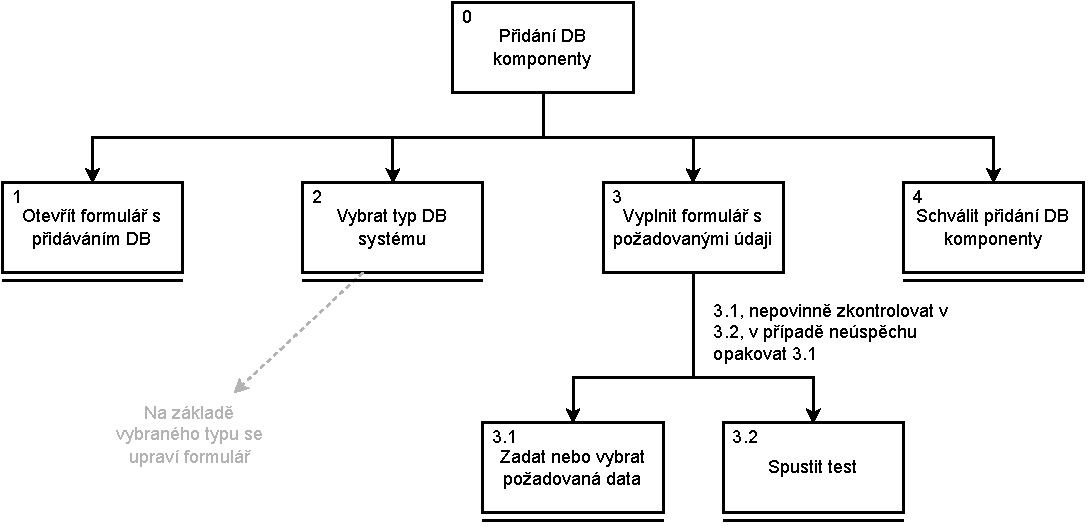
\includegraphics[height=70mm]{../img/HTA-1}
  \caption{Diagram pro přidání databázové komponenty.}
  \label{obr03:hta1}
\end{figure}

Kořen oznamuje jaký úkol bude uživatel provádět. V~první hladině máme kroky 1 až 4, které nám v~základních rysech ukazují, jak bude uživatel postupovat při plnění úkolu. Krok 3 dál rozdělíme na 3.1 Zadání dat a~3.2 Otestování. Na hraně pak definujeme postup uživatele při plnění kroků 3.1 a~3.2. Když není hrana popsaná, předpokládáme průběh kroků podle čísel v~hladině vzestupně. Konkrétní pořadí ale není podmíněné. Číslování 3 a~3.x vyjadřuje vztah mezi rodičem a~podúkoly.  Podtržené stavy v~HTA se dál nedělí. 

Takto vytvořený diagram nám neříká nic o~interakci uživatele s~konkrétním systémem. Díky tomu ale můžeme kroky rychle měnit a~upravovat. Lépe zhodnotíme, jestli uživatel nedělá příliš mnoho kroků pro dokončení úkolu, nebo naopak. Často se může stát, že jeden krok je ještě potřeba rozdělit.

Všechny tři analýzy úkolů, včetně přidání DB komponenty jsou k nahlédnutí v příloze \ref{priloha1}.
